\documentclass[a4paper]{scrartcl}

\usepackage[utf8]{inputenc}
\usepackage[english]{babel}
\usepackage{lmodern} 
\usepackage[T1]{fontenc}
\usepackage{booktabs}
\usepackage{multirow}
\usepackage{wrapfig}


% PAKETE
\usepackage{siunitx}
\usepackage{graphicx}
\usepackage{placeins}
\usepackage{longtable}
\usepackage{enumitem}
\usepackage{bbm}
%\usepackage{sidecap}


\usepackage{amssymb} % math symbols
\usepackage{amsmath} % ams
\usepackage{amsfonts} % mathmatical fonts

% caption indenting
 \usepackage[format=plain,indention=0em,labelfont=bf,margin=1em]{caption} 
 \usepackage{subfig} %subfigures ^^
\usepackage[protrusion=true,expansion=true]{microtype} % denser font, "-" behind line
\usepackage{esint} % nicer double and triple integrals
\usepackage{fancyhdr} % fancy headers
\usepackage[colorlinks=true,linkcolor=black,citecolor=black,filecolor=black,urlcolor=black]{hyperref}



% EINSTELLUNGEN
\sisetup{seperr,repeatunits=false}
\numberwithin{equation}{section}
\numberwithin{figure}{section}
\numberwithin{table}{section}

% EIGENE FUNKTIONEN
\newcommand{\re}{\operatorname{Re}}
\newcommand{\im}{\operatorname{Im}}
\newcommand{\gquote}[1]{\glqq #1 \grqq}

\newcommand{\eq}[2]{\begin{equation}#1\label{#2}\end{equation}}
\newcommand{\eqand}[0]{\hspace{.25cm} \bigwedge \hspace{.25cm}}
\newcommand{\grafik}[2]{\begin{figure}[h]\centering \includegraphics[width=10cm]{#1.eps}  \caption{#2} \label{#1} \end{figure} }
\newcommand{\grafikq}[3]{\begin{figure}[h]\centering \includegraphics[width=10cm]{#1.eps}  \caption[#2]{#3} \label{#1} \end{figure} }
\newcommand{\tbl}[3]{\begin{table}[h]\caption{#1}\label{#2}\begin{center}#3\end{center}\end{table}}
\newcommand{\Abbildung}[1]{\textsl{Abbildung \ref{#1}}}
\newcommand{\AbbildungI}[1]{\textsl{(Abbildung \ref{#1})}}
\newcommand{\Tabelle}[1]{\textsl{Tabelle \ref{#1}}}
\newcommand{\TabelleI}[1]{\textsl{(Tabelle \ref{#1})}}
\newcommand{\Formel}[1]{(\ref{#1})}
\renewcommand{\d}{\mathrm{d}}
\newcommand{\ve}[1]{\mathbf{ #1} }

\title{Ma 4: X-Ray Photoelectron Spectroscopy (XPS)}
\subtitle{Tutor: B. Zhang}
\author{Benjamin Huber, Carolin Wille}
\date{December 12, 2011}

\begin{document}
\thispagestyle{empty}
\maketitle
\tableofcontents
\clearpage


\section{Introduction}
X-Ray Photoelectron Spectroscopy (XPS) is a spectroscopic technique, which can be used to analyze the fundamental electronic processes and structures in atoms, molecules or solids. As suggested by the name, x-rays are shot at a sample, inducing various processes, that lead to the emission of electrons. The electronic spectrum is resolved with respect to the kinetic energy and yields information about core levels, the valence band and the Fermi energy, as well as plasmons and the Auger process. However XPS is quite surface sensitive due to the relatively small escape depth of electrons, which depends on their energy and is determined by the so called universal curve shown in figure \ref{fig:uni}. The energy range of a typical XPS spectrum is from $\SI{200}{eV}$ to $\SI{1600}{eV}$, thus the typical mean-free path of the electrons varies from $2 \AA $ to $20 \AA$. In order to analyze the sample and not adsorbed layers of gas, e.g. oxygen superstructures, it is necessary to work in ultra-high vacuum (UHV).
\begin{wrapfigure}{r}{0.6 \textwidth}
  \centering
   	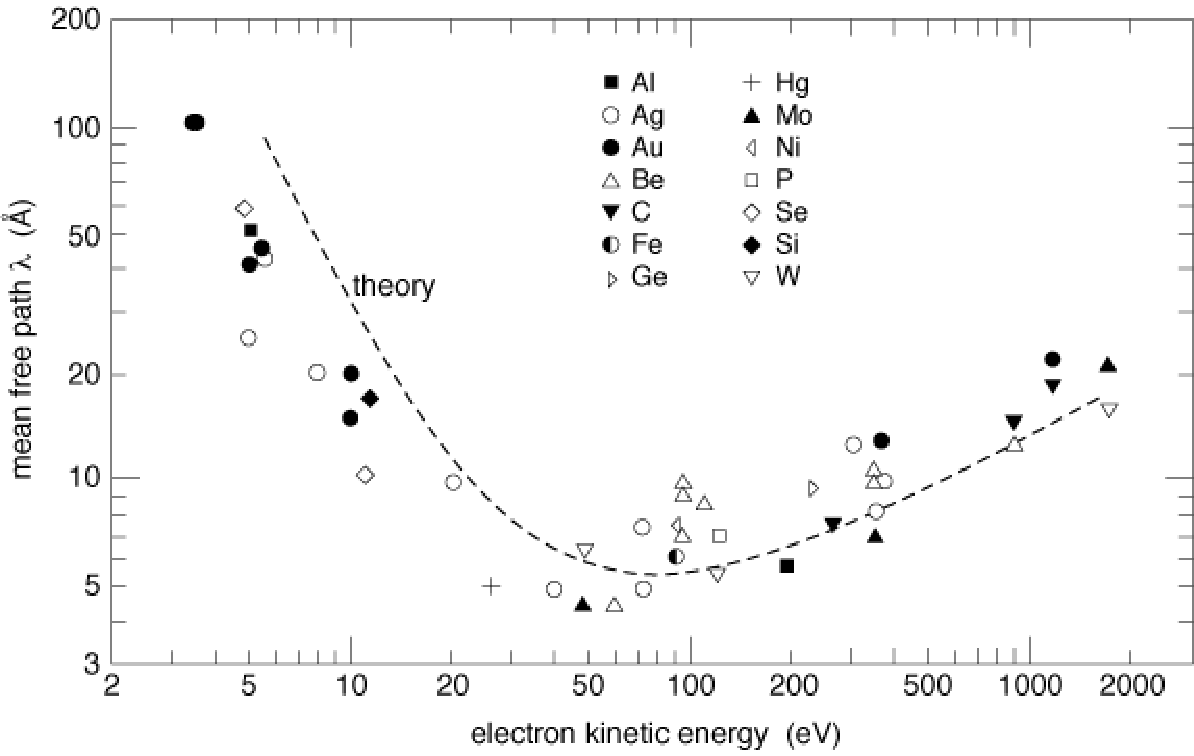
\includegraphics[width=\linewidth]{img/meanfree.pdf}
 \caption{\small Universal curve of solids \cite{zangwill}.  }
        \label{fig:uni}
\end{wrapfigure}


\FloatBarrier
\subsection{Energy Spectrum}
To understand the full spectrum of XPS it is necessary to understand each individual processes involved to be able to differentiate the peaks and draw any conclusion from their locations.


\subsubsection{Photoelectric Effect}
The most obvious contribution to the XPS spectrum is that of the photoelectric effect. A single electron absorbs the photon of energy $h\nu$, leaving the sample with a remaining energy of
\eq{E_\text{kin} = h\nu - E_\text{B} - \Phi \, ,}{}
where $E_\text{B}$ is the binding energy of this electron (relative to the Fermi energy) and $\Phi$ the work-function (minimum energy needed to remove an electron from a solid).
As there are only electrons in the atom up the the Fermi energy $E_\text{F}$, there are no electrons to be detected for (kinetic) energies greater than $h\nu -\Phi$. Typically this is used to define all measured energies relative to this Fermi energy.

This binding energy is not equal to the binding energy of the electron in a free atom. Bonds with the neighbouring atoms (chemical shift $\Delta E_\text{chem}$), electrostatic interaction with the whole lattice (Madelung constant $\Delta E_\text{Mad}$) and many-body effects of the hole in the final state (relaxation effects $\Delta E_\text{rel}$) influence the measured energy
\eq{E_\text{B}=E_\text{B,free} + \Delta E_\text{chem} + \Delta E_\text{Mad} + \Delta E_\text{rel} \; . }{}

\subsubsection{Spin-orbit Coupling and Multiplet-Structures}
The interaction between the spins of the electrons and their angular momenta, the so called spin-orbit-coupling leads to the splitting of energy niveaus within one shell. In general there are two different types of spin-orbit coupling, distinguished by the dominant coupling effect, which is either the coupling between all electronic angular momenta and all electron spins (LS-Coupling) or between the angular momentum and the spin of each electron separately ($jj$-Coupling). The latter case is relevant in this experiment and its single electron Hamiltonian is given by
\eq{H=a \ve s \cdot \ve l\;,}{hamilton}
where $\ve l$ is the angular momentum of the electron, $\ve s$ the spin and $a$ is the coupling constant. The eigenstates with energy shifts
\eq{\Delta E_{sl} = a [(j(j+1)-l(l+1)-s(s+1)]}{spinorbitE}
are then characterized by the total angular momentum, which can have the values $(l+\tfrac 1 2)$, $(l - \tfrac 1 2)$ except for the $s$-shell ($l=0$), where no coupling effects between angular momentum and spin can occur. However, it was found by Abragam \cite{Abragam} and experimentally verified, that the degeneracy of the fully filled $s$-state can be lifted by the interaction with another partially filled shell yielding again a two-folded splitting (doublet). This effect is called magnetic spin-spin exchange.


\subsubsection{Auger Process}
When there is an electron missing in one of the inner shells of the atom, another electron from an higher shell will take its place. During this process either a photon will be emitted directly or the energy will be transferred to a third electron which now has enough energy to leave the atom. This latter process is called the Auger process. As XPS will remove electrons from the inner shells as well as the outer shells, this process will cause additional peaks in the spectrum. It is customary to label the Auger peaks with the shell-labels of the three electrons involved (eg. KLL for missing electron in the first shell, filling and leaving electron from the second shell). The positions of the Auger peaks are specific for the material being investigated.

The energy balance of the Auger-transition reads
\eq{E(KLL') = E(K) -E(L) - E^{*}(L') \; ,}{EKLL}
where $E(KLL')$ is the energy of the Auger electron stemming from a transition KLL', E(K)/E(L) are the binding energies of the electrons of the K/L-level and $E^*(L')$ is the binding energy of the electron in the $L'$ state, where the asterisk denotes, that this energy is altered through the absence of the $K$ and $L$ electron.

These formulas hold for free atoms. For an electron, that is emitted from the valence band of a solid the work-function has to be taken into account.


\subsubsection{Plasmons}
\label{sec:plasmonIntro}
The pseudo particle of fermi-gas oscillation is called a plasmon. These plasmons have characteristic energies, depending on the conduction electron density $n$. 
$$E_p = \hbar \underbrace{\sqrt{\frac{ne^2}{m_e \epsilon_0}}}_{\omega_p}$$
Eg. a calculation for aluminum, which has a conducting electron density of $n=1.8 \times 10^{29} \text{m}^{-3}$ yields $E_p(Al)=15.8 \text{eV}$.
Apart from the more obvious bulk plasmons (three dimensional oscillations in the sample) there are also surface plasmons when a material with positive dielectric constant (vacuum) interfaces with a material of negative dielectric constant (metal). Exact values for both bulk and surface plasmon energies for different materials are known in principle and can be looked up in the appropriate literature.

An electron that excites a plasmon looses one of these characteristic energies and is said to have suffered plasmon loss. It is possible, that one electron suffers plasmon loss several times, leading to a series of equally spaced losses with decreasing intensity.


\subsubsection{Shake-Up and Shake-Off}
%Impurities and lattice effects allow many-body interactions that would be impossible in a single atom. %??
Shake-up and shake-off events will divide the energy of the incoming photon between two electrons. Either one electron is emitted, leaving the atom in an exited state (shake-up) or both electrons are emitted (shake-off). Both effects depend on the energy levels of the atom and are thus characteristic for the material but are not as easily quantized as the other effect stated above.

Because the shake-off event can happen with even more than two electrons, it may lead to broad structures at the low kinetic (or high binding) energies of the spectrum.


\subsubsection{Satellite Peaks}
If the x-ray source is not monochromatic, there will be so called satellite peaks. The distance to the main peak and their intensity depends on the energy difference and relative intensities of the harmonics in the anode material of the x-ray source.

\clearpage


\subsection{Experimental Set-Up and Measurement Procedures}

In the experiment an X-Ray source (cf. fig. \ref{fig:setup} \textbf{(b)}) emits photons, which hit the sample. The photo-electrons are detected by an analyzer and the whole set-up is placed in vacuum (cf fig. \ref{fig:setup} \textbf{(a)}).


\begin{figure} 
 \centering
 \subfloat[][Set-Up]{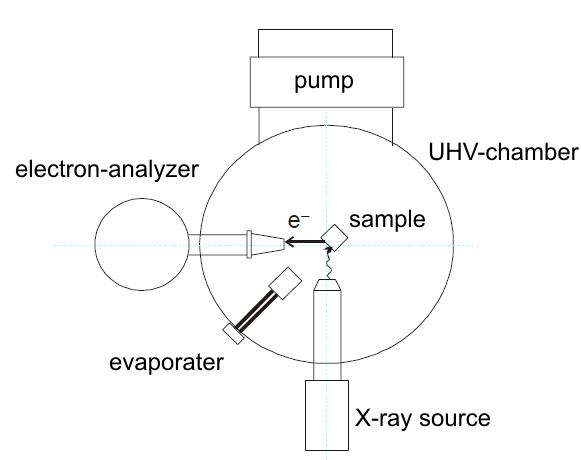
\includegraphics[width=0.45\textwidth]{img/setup.png}}
 \hfill
  \subfloat[][X-Ray Source]{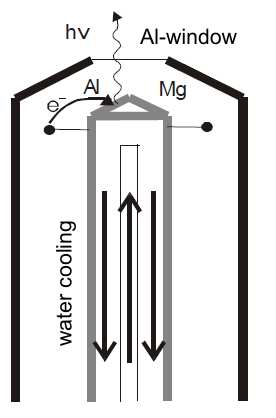
\includegraphics[width=0.25\textwidth]{img/xray.png}}

\caption{ \small \textbf{(a)} Schematic Description of the Experimental Set-Up. \textbf{(b)} Double-Anode X-Ray-Source: An Aluminum window blocks low energetic photons (Bremsstrahlung). Mg (Mg-$K_\alpha=1253.6\pm 0.7\,\text{eV}$) and Al (Al-$K_\alpha=1486.6\pm 0.6\,\text{eV}$)  can be used as sources. Source: \cite{script} } 
	\label{fig:setup}
\end{figure}

\FloatBarrier

\subsubsection{Ultra High Vacuum (UHV)}
As the electrons interact with all kind of materials, it is very useful to operate in high vacuum. This is also necessary in order to reduce the rate of adsorption of molecules, which leads to disturbance of the measured spectra. (Ultra) high  vacuum (UHV) can only be achieved by a series of pumps acting within different pressure ranges.
\begin{wraptable}{r}{0.55\textwidth}
\begin{tabular}{lr}
\toprule
pump & pressure range (Pa)\\
\midrule
\small rotary vane pump & $10^5$ - $10^{-1}$  \\ 
\small turbo molecular pump &  $10^0$  - $10^{-9}$  \\
\small ion getter pump  & $ 10^{-3}$  - $10^{-9}$  \\
\small titan sublimation pump & $10^1$  - $10^{-9}$  \\
\bottomrule
\end{tabular}
\caption{Different pumps and their pressure operating range. \cite{gop} }
\label{tab:pump}
\end{wraptable}


\subsubsection*{Rotary vane pump}
The rotary vane pump is a simple mechanical pump, which consists of a cylinder connecting the vacuum cell and the outer space. In the cylinder a vane rotates and thereby shovels the gas to the outside. Springs ensure optimal contact between the vane and the cylinder walls. 
\begin{figure} 
 \centering
\subfloat[][Rotary vane pump]
{        	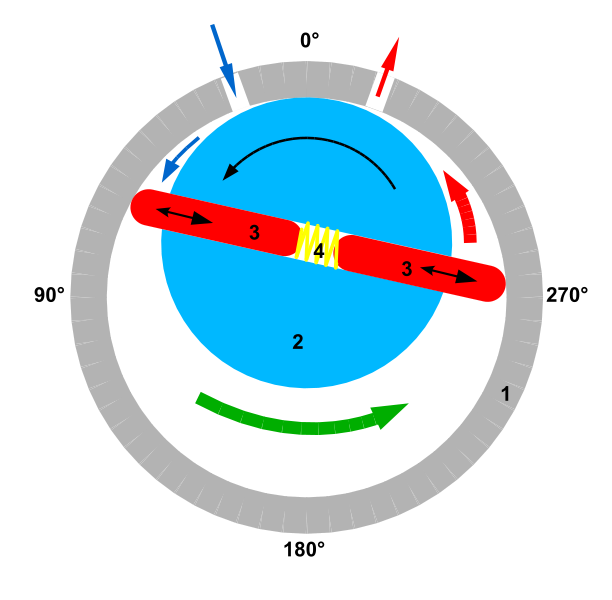
\includegraphics[width=0.45\textwidth]{img/rot.png}}
 \hfill
\subfloat[][Turbomolecular pump]
         { 	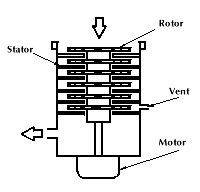
\includegraphics[width=0.45\textwidth]{img/tu.jpg}}
\caption{
\small \textbf{(a)} Rotary vane pump. 1: pump housing, 2: rotor, 3: vanes, 4: spring,  \textbf{(b)} Schematic description of a turbomolecular pump } 
	\label{fig:pump}
\end{figure}


\subsubsection*{Turbomolecular pump}
The main features of a turbomolecular pump are the rotating blades (rotors), hitting the molecules very often per unit time, thereby enforcing a velocity distribution within the gas that is not isotropic, but a certain direction is preferred. Within the pump there are other static blades (stators), which act as a kind of filter to the velocity of the molecules in such a way, that molecules with the velocity, that is predominantly created by the rotors, can pass through with a higher probability. These filters act only in one-way, so that the molecules stay on the other side as long as the asymmetric velocity distribution is maintained. 


\subsubsection*{Baking}
The above mentioned pumps can reach pressures of down to $10^{-9}\,\text{Pa}$ (cf. table \ref{tab:pump}). The remaining pressure, which is mainly due to the water molecules sticking to the walls of the chamber, can be lowered by thermal methods called baking. When the heated chamber with a pressure of still $10^{-9}\,\text{Pa}$ (due to the pumps still being active) is cooled down again, pressures of below $10^{-11}\,\text{Pa}$ can be reached. This process can take several days, so it is paramount to keep the pressure at this low level during and in between experiments.

\clearpage
\subsubsection{Electron Energy Analyzer}

\begin{wrapfigure}{r}{0.6 \textwidth}
  \centering
   	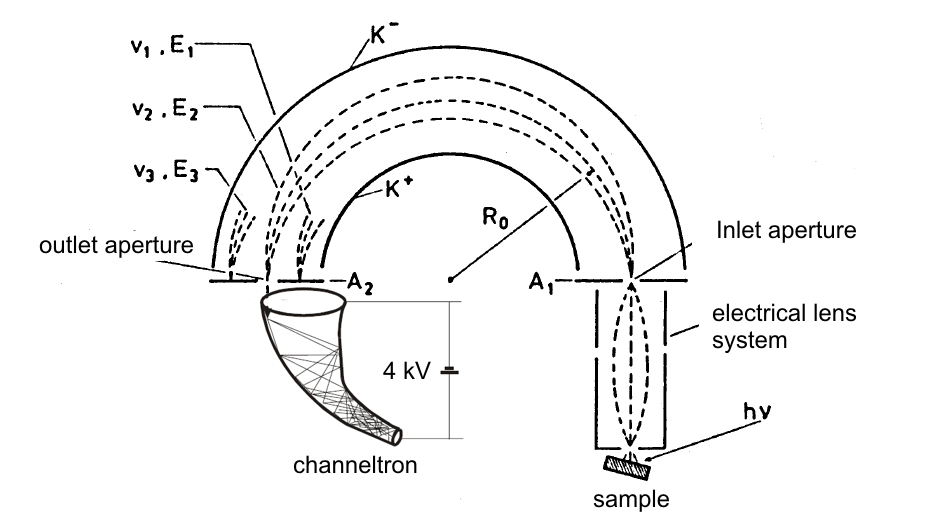
\includegraphics[width=\linewidth]{img/channeltron.png}
 \caption{\small Electron Analyzer consisting of electronic lens system, hemispheric capacitor as energy filter and channeltron. Source: \cite{gop} }
        \label{fig:analyzer}
\end{wrapfigure}
The electron energy analyzer is the central measurement device, as it performs the resolution of electron numbers with vs. energy. In this experiment a concentric hemispheric capacitor is used as an energy filter (cf. fig. \ref{fig:analyzer} b). The trajectory of the electron is altered by the electric field of the capacitor, in such a way, that only electrons with a certain range of kinetic energy can pass the analyzer. This pass energy can be chosen by applying appropriate voltage. Before entering the analyzer, the electrons are focussed by an electrical lens system and after they exit the analyzer are detected by a channeltron, that works as an electron multiplier (factor $10^6$ to $10^8$) and produces analog signals, which can be digitalized and processed by a computer. 

\clearpage
\section{Analysis}
\subsection{Spectrum of a silver sample}
A silver sample is investigated with a magnesium and an aluminum x-ray filament at the photon energies Mg-$K_\alpha=1253.6 \pm 0.7\,\text{eV}$ and Al-$K_\alpha=1486.6\pm 0.6 \,\text{eV}$. Figure \ref{fig:compare} shows both spectra in comparison. Most characteristic features of the spectra are shifted by the difference of the photon energy of about $230$ eV, which is expected for peaks originating from core-level transitions. Additionally at about $350$ eV there are peaks in both spectra, which can be identified as Auger peaks, as the Auger electron energy does not depend on the primary excitation source.

\begin{figure}
  \centering
   	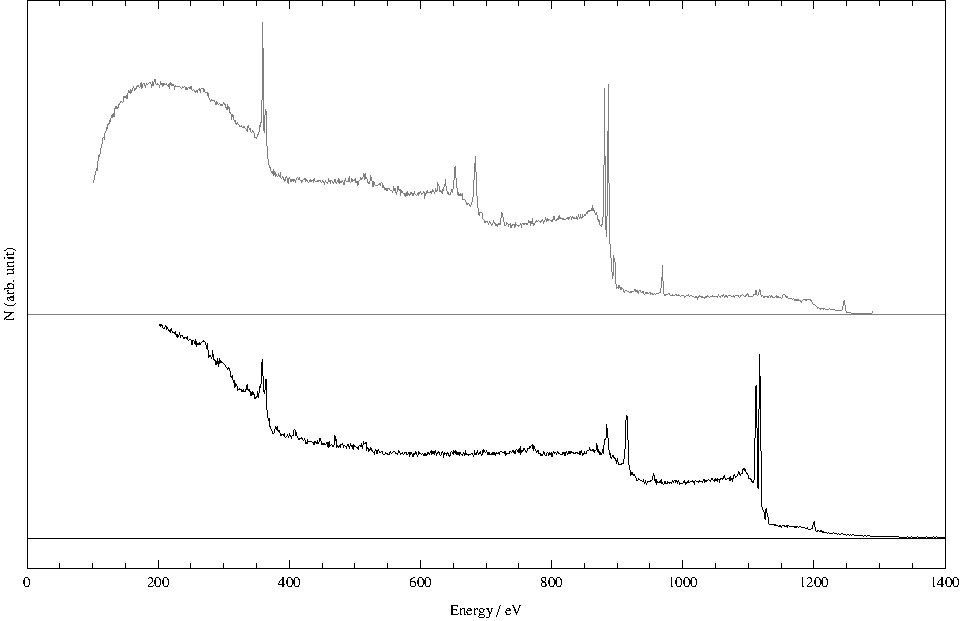
\includegraphics[width=0.75\linewidth]{img/compare.pdf}
 \caption{\small Ag-Spectra excited by Mg-$K_\alpha$ (top, gray) and Al-$K_\alpha$ (bottom, black) x-rays.  }
        \label{fig:compare}
\end{figure}

In order to generate a spectrum with respect to the binding energy, the Fermi energies for both spectra are determined (Al: $1479.5 \pm 0.5 \,\text{eV}$, Mg: $1249.0\pm 0.5 \,\text{eV}$). Figure \ref{fig:agfermi} shows a close-up of the Fermi region, from which it can be seen, that the determination of the Fermi energy can not be done with high precision. In figure \ref{fig:agal} and \ref{fig:agmg} the binding energy spectra are displayed and all peaks, that could be matched are labeled. The peaks were found by fitting Lorentzians (Cauchy-distributions) around the maxima after a linear noise level was subtracted. For most peaks, the positions in the spectra generated with the two different x-ray sources are very similar. However, there are peaks, which do not match well, i.e. the 3s peak. Additionally to the core transitions, some additional plasmon excitations (denoted '+P') and the Auger peak, impurities of carbon and oxygen could be detected in the spectrum. There are some remaining peaks, which could not be matched to either of the latter processes. These peaks most probably result from shake-up/shake-off processes.
The core transition correspond to binding energies, which are compared to literature values. For the Auger electron it is more sensible to compare the absolute electron energies.
\begin{table}
\centering
\begin{tabular}{lrr}
\toprule
$E_\text{Al}$ (Auger) in eV & $E_\text{Mg}$ (Auger) in eV  & $E_\text{literature}$ ( $3d_{5/2}$) in eV  \\
\midrule
 $359.0 \pm 0.5$ &$ 359.5 \pm 0.5$ & 368.22 \\
 \bottomrule
 \end{tabular}
 \caption{ \small Auger Electron Energy of the Ag $3d_{5/2}$ electron compared to literature.\cite{augerpaper}}
 \label{tab:auger}
\end{table}



\begin{table}
\centering
$
\begin{array}{lrrr}
\toprule
\text{peak} & E_B \text{in eV (Al)}  &  E_B \text{in eV (Mg)} & \text{Literature} \cite{handbook} \\
\midrule
\text{Ag(Auger)} &  1120.31 \pm 1.34 &  889.60 \pm 0.60 &-\\
\text{Ag(3s)} &  710.16 \pm 2.08 &  735.09 \pm 1.31 &719.0\\
\text{Ag}(3p_{1/2}) & 595.33 \pm 0.69 &   596.20 \pm 0.57 &603.8 \\
\text{Ag}(3p_{3/2}) & 564.93 \pm 0.55 &   565.39 \pm 0.53  & 573.0\\
\text{O(1s)} & 523.90 \pm 0.57 &  524.46 \pm 0.62 &  543.1 \\
 \text{Ag(3d)+P} & 386.15 \pm 1.25 & 386.61 \pm 0.98  &-\\
\text{Ag}(3d_{3/2}) & 367.61 \pm 0.78 &  368.37 \pm 0.51 & 374.0 \\
\text{Ag} (3d_{5/2}) &  361.96 \pm 1.05 & 362.48 \pm 0.54 & 368.3 \\
 \text{C(1s)} & 279.31 \pm 0.67 &  280.06 \pm 0.53 & 284.5 \\
\text{Ag(4s)} & 94.37 \pm 2.61 &  93.54 \pm 0.79 & 97.0 \\
\text{Ag(4p)} & 55.91 \pm 1.19 & 56.19 \pm 0.67  & 63.7 (1/2), 58.3 (3/2) \\
 \text{Ag(4d)} & 2.61 \pm 0.52 &  3.04 \pm 0.52 & 4.5 \\
 \bottomrule
\end{array}
$
\caption{
\small Spectrum of Ag generated by Al-$K_\alpha$ x-rays and Mg-$K_\alpha$ x-rays compared to literature values.   } 
	\label{fig:tabelle}
\end{table}



\subsection{Samarium (Sm) spectrum}
\subsubsection{Overview Spectrum}
A Samarium (Sm) sample was investigated with the Al-$K_\alpha$ x-ray source. To this end a fresh Samarium film was evaporated on the sample for about 30 minutes. The Fermi energy was determined to be $1479.5\pm 0.5 \,\text{eV}$ and the matching of the peaks was done as described in the previous section. The results of the overview spectrum analysis are listed in figure \ref{fig:sm}.


\FloatBarrier
\subsubsection{3-d Spectrum}
The 3-d spectrum of Samarium is investigated with subject to two different phenomena. Firstly, the multiplet splitting caused by spin-orbit interaction is analyzed and secondly, the occurrence of satellite peaks due to the different valence-states in the bulk and on the surface is examined. The spin-orbit multiplet splitting is clearly visible in figure \ref{3d} and the binding energy difference of $\Delta E_{d_{3/2}d_{5/2}} = 27.1 \pm 0.5 \,\text{eV}$ between the $3d_{3/2}$ and $3d_{5/2}$ peak is in close agreement to the values given in literature $\Delta E_{d_{3/2}d_{5/2}}^{\text{ref}}$ as e.g. measured by  G. K. Wertheim et al. \cite{wertheim}. With the values ${j=5/2, s=1/2, l=2}$ and ${j=3/2, s=1/2, l=2}$ the energy spacing can be calculated using equation \Formel{spinorbitE}, which gives $\Delta E_\text{calc}=\lvert-3/2 a - a \rvert=5/2 a$. The coupling constant can thus be determined to be 
\eq{a=10.5\pm 0.2\,\text{eV} \; .}{a}
The electron configuration of Samarium is [Xe]$6s^24f^6$, which implies, that the 3d shell is fully populated. According to the Pauli principle, there are 5 electron with spin up and 5 with spin done, hence the intensities of the two 3d peaks should be equal. This can be confirmed by integrating of the two peaks. To this end, the peaks were fitted with Voigt profiles (product of Gaussian and Lorentzian functions) and a linear noise level was subtracted (visualized in fig \ref{3d}). The subsequent (improper) integration of the Voigt functions (over the whole energy range) without noise resulted in a relation of 97600:97400.

The satellite peak in the 3d spectrum is a surface phenomenon. On the surface, a divalent state is favored over the usual trivalent state, because of surface tension forces  \cite{johansson}. The lowering of energy is visible in the 3d multiplet, where both peaks show satellite peaks at about 7.6 eV \cite{wertheim} lower bindings energies. However, in our spectrum this satellite peak is only visible at the $3d_{5/2}$ peak, but the distance of $10.3 \pm 0.5 \,\text{eV}$ is in qualitative agreement with the literature. The invisibility of the $3d_{3/2}$ peak is due to the noise level, which is rapidly increasing with decreasing kinetic energy of the electron (corresponding to higher binding energies). For the same reason, we decided to use the Al-filament, which has a higher x-ray energy and thus produces electrons at a higher kinetic energy compared to the Mg-filament. If it was not for this noise increase at lower kinetic energies, we would have chosen the Mg filament, because the lower kinetic energy would have lead to a more dominant impact of surface effects resulting from the decreased escape depth (see universal curve \ref{fig:uni}).

The spectrum was taken for different pass energies varying from \SI{20}{eV} to \SI{100}{eV} in order to obtain the best results in a compromise between noise level and the linewidth of the peaks. Best results were achieved at a pass energy of \SI{50}{eV}.  


\subsection{Spectrum and Components of a 10 DM (Deutsche Mark) Coin}
A 10 DM coin was investigated with the Al filament in order to study its elemental composition. However, the coin was highly contaminated with Samarium, which had been evaporated in the chamber before. The coin should be made of $92.5 \%$ silver and $7.5\%$ copper or $62.5 \%$ silver and $37.5 \%$ copper depending on the specific memorial coin \footnote{\url{http://de.wikipedia.org/wiki/Liste_der_Gedenkmünzen_der_Bundesrepublik_Deutschland _(DM)}}. A comparison with an xps spectrum of copper from the National Physics Laboratory \cite{npl} shown in figure \ref{fig:DM}c shows, that it is not at all surprising, that only the 2p core transition peaks of copper could be found within the spectrum of the coin as their intensities are much higher than those of all other core transitions. The detection of these peaks is therefore all that can be expected to validate the copper within the coin. Several silver core level transitions could also be detected within the spectrum as well as the oxygen and carbon impurities, that were present in the other spectra as well.


\section{Summary and Discussion}
Silver, samarium and an unknown sample were investigated with X-Ray Photoelectron Spectroscopy. All significant peaks (including Auger peaks) were located in the silver and samarium sample with radiation from both a Mg source and an Al source.

A detailed measurement of the 3-d region of the samarium sample confirmed the 1:1 ratio of the two peaks and one of the two satellite peaks was observed as expected.

While the relative spacing underlines the correctness of the mapping of peaks to transitions, the absolute values for the binding energies to not correspond to the literature values. The discrepancy increases with higher binding energies and points towards a systematic error in the experimental setup such as tilted samples, charged samples or an inaccurate spectrometer.

Nonetheless the discrepancies were consistent over several measurements such that it was possible to identify the peaks in the spectrum of the memorial coin. Most of them were samarium peaks, but it was still possible to identify copper and silver in the coin. Due to the high degree of contamination with samarium it is likely, that it accumulated over the course of several experimental groups. An intermediate sputtering or filing of the sample would have greatly increased the quality of the spectrum.





\clearpage
%----------------------------------- Fermi ------------------------------
\begin{figure}
\section{Spectra}
  \centering
   	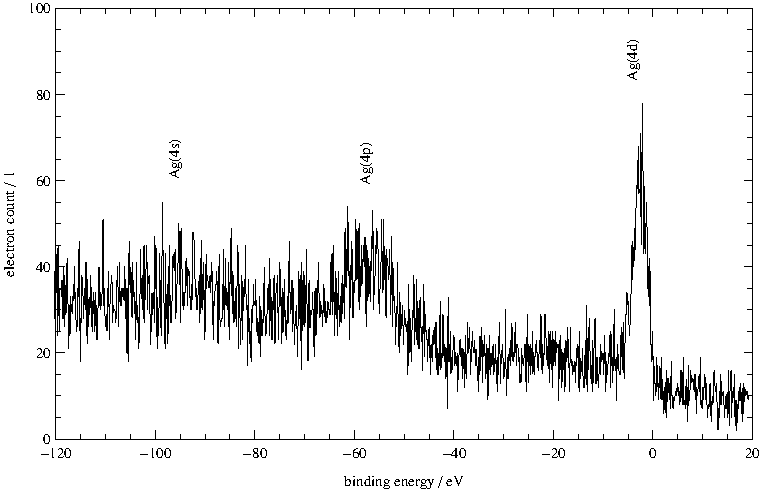
\includegraphics[width=\linewidth]{img/AgAlFermi.pdf}
 \caption{\small Region of the Ag spectrum near the Fermi energy (Al filament).}
        \label{fig:agfermi}
\end{figure}
% ----------------------------------- Al -----------------------------------
\begin{figure}[p] 
 \centering
\subfloat[][Spectrum]
{  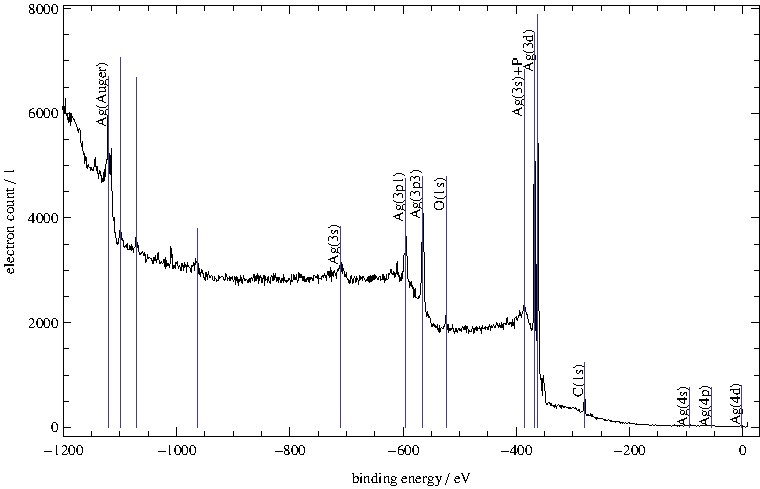
\includegraphics[width=\linewidth]{img/agalwtf.pdf} }       \hfill %
\subfloat[][Peak positions]  %     
{ \small  $
\begin{array}{rr}
\toprule
E_B \text{in eV (Al)}  & \text{assigned peak} \\
\midrule
 1209.55 \pm 1.45 & \text{} \\
 1120.31 \pm 1.34 & \text{Ag(Auger)} \\
 1099.24 \pm 0.96 & \text{} \\
 1069.95 \pm 1.69 & \text{} \\
 963.60 \pm 1.14 & \text{} \\
 710.16 \pm 2.08 & \text{Ag(3s)} \\
 595.33 \pm 0.69 & \text{Ag}(3p_{1/2}) \\
 564.93 \pm 0.55 & \text{Ag}(3p_{3/2}) \\
 523.90 \pm 0.57 & \text{O(1s)} \\
 386.15 \pm 1.25 & \text{Ag(3d)+P} \\
 367.61 \pm 0.78 & \text{Ag}(3d_{3/2}) \\
 361.96 \pm 1.05 & \text{Ag}(3d_{5/2}) \\
 279.31 \pm 0.67 & \text{C(1s)} \\
 94.37 \pm 2.61 & \text{Ag(4s)} \\
 55.91 \pm 1.19 & \text{Ag(4p)} \\
 2.61 \pm 0.52 & \text{Ag(4d)} \\
 \bottomrule
\end{array}
$
}
\caption{\small Ag-Spectrum excited by Al-$K_\alpha$ x-rays. Core transitions, satellite and peaks resulting from impurities (C,O) could be detected and are compared to literature values \cite{handbook}. }
  \label{fig:agal}
\end{figure}

\begin{figure}[p] 
 \centering
\subfloat[][Spectrum]
{  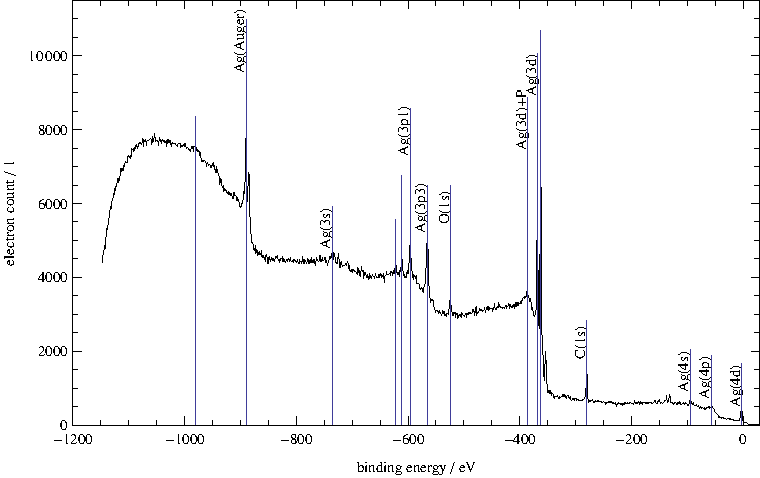
\includegraphics[width=\linewidth]{img/agmgwtf.pdf} }       \hfill %
\subfloat[][Peak positions]  %     
{ \small  $
\begin{array}{rr}
\toprule
E_B \text{in eV (Mg)}  & \text{assigned peak} \\
\midrule
 980.47 \pm 1.50 & \text{} \\
 889.60 \pm 0.60 & \text{Ag(Auger)} \\
 735.09 \pm 1.31 & \text{Ag(3s)} \\
 622.00 \pm 0.87 & \text{} \\
 610.94 \pm 0.60 & \text{} \\
 596.20 \pm 0.57 & \text{Ag}(3p_{1/2}) \\
 565.39 \pm 0.53 & \text{Ag}(3p_{3/2}) \\
 524.46 \pm 0.62 & \text{O(1s)} \\
 386.61 \pm 0.98 & \text{Ag(3d)+P} \\
 368.37 \pm 0.51 & \text{Ag}(3d_{3/2}) \\
 362.48 \pm 0.54 & \text{Ag}(3d_{5/2}) \\
 280.06 \pm 0.53 & \text{C(1s)} \\
 93.54 \pm 0.79 & \text{Ag(4s)} \\
 56.19 \pm 0.67 & \text{Ag(4p)} \\
 3.04 \pm 0.52 & \text{Ag(4d)} \\
% -5.64 \pm 0.56 & \text{sat} \\
 \bottomrule
\end{array}
$ 
}
\caption{\small Ag-Spectrum excited by Mg-$K_\alpha$ x-rays. Core transitions, satellite and peaks resulting from impurities (C,O) could be detected and are compared to literature values \cite{handbook}. }
  \label{fig:agmg}
\end{figure}

%------------------------------ Sm ----------------------------------
\begin{figure}[p] 
 \centering
\subfloat[][Spectrum]
{  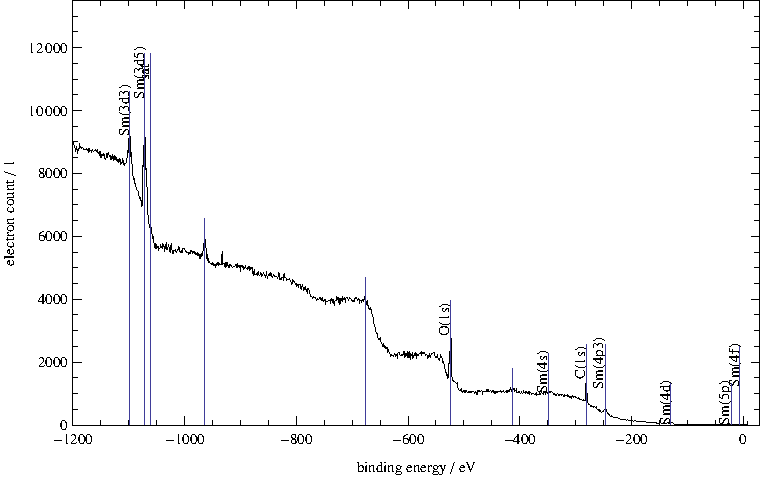
\includegraphics[width=\linewidth]{img/smwtf.pdf} }       \hfill %
\subfloat[][Peak positions]  %     
{ \small  \begin{tabular}[b]{lrr}
 \toprule
\text{peak} & $E_B$ \text{in eV}  & Literature  \\
\midrule
Sm(3$d_{3/2}$) & $1098.35 \pm 0.50 $& 1110.9 \\
 Sm(3$d_{5/2}$) &$ 1071.24 \pm 0.51$ & 1083.4\\
\text{sat}  &$1060.90 \pm 0.55$ &  -\\
\text{} &$964.03 \pm 0.59$ &  -\\
\text{}& $675.30 \pm 1.28 $& -\\
 \text{O(1s)}& $523.59 \pm 0.67 $& 543.1 \\
\text{} &$412.39 \pm 1.79 $&  -\\
\text{Sm(4s)}& $347.96 \pm 2.6$ & 347.2 \\
\text{C(1s)} &$281.01 \pm 0.54$ &  284.5\\
Sm(4$p_{3/2}$) &$246.56 \pm 0.71$ &  247.4\\
\text{Sm(4d)} &$130.11 \pm 0.99$ &  129\\
\text{Sm(5p)} &$20.43 \pm 0.68 $&  21.3\\
\text{Sm(4f)} & $6.55 \pm 0.65 $&  5.2 \\
 \bottomrule
\end{tabular}
}
\caption{\small Sm-Spectrum excited by Al-$K_\alpha$ x-rays. Core transitions, satellite and peaks resulting from impurities (C,O) could be detected and are compared to literature values \cite{handbook}. }
  \label{fig:sm}
\end{figure}
%--------------------------------- Sm3d -----------------------------------
\begin{figure}
  \centering
   	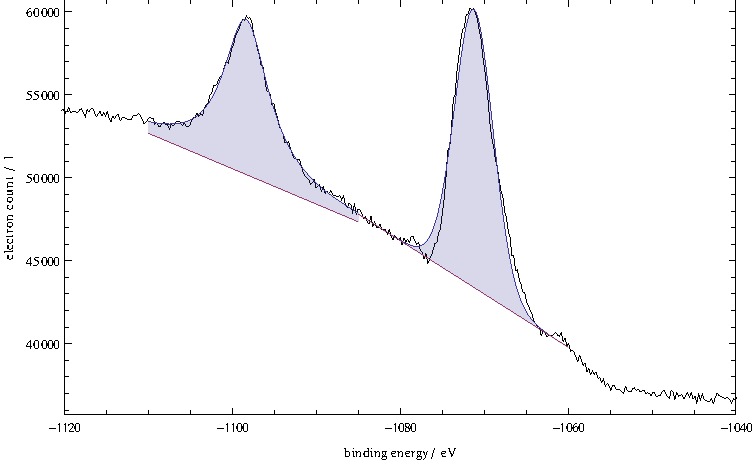
\includegraphics[width=\linewidth]{img/3d.pdf}
 \caption{\small Samarium 3d spectrum showing the multiplet splitting and one satellite peak due to divalent surface state. }
        \label{3d}
\end{figure}
% ------------------------------------ DM -----------------------------------
\begin{figure} 
 \centering
\subfloat[][spectrum of a 10 DM memorial coin]
{  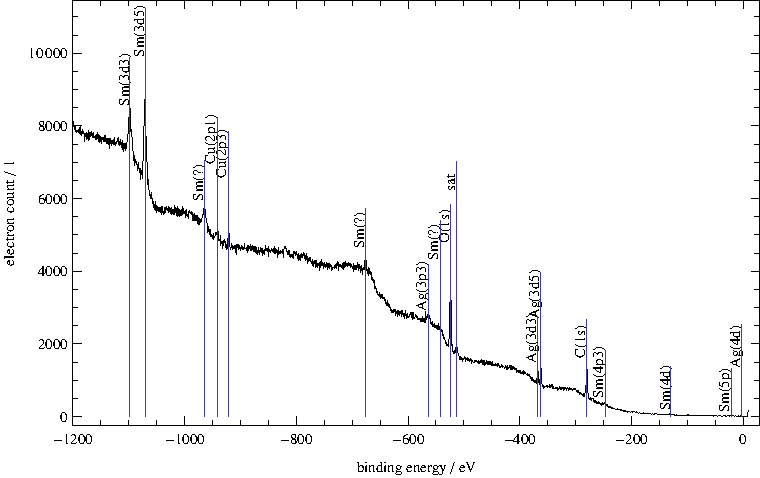
\includegraphics[width=\linewidth]{img/DM.pdf} }       

\subfloat[][peak positions] {
\begin{tabular}[b]{rr}
 \toprule
$E_B$ \text{in eV}  & \text{peak} \\
\midrule
$ 1098.05 \pm 0.55$ & \text{Sm(3d3)} \\
 $1070.92 \pm 0.53 $& \text{Sm(3d5)} \\
 $964.39 \pm 0.64 $& \text{Sm(?)} \\
 $940.97 \pm 0.65 $& \text{Cu(2p1)} \\
 $921.38 \pm 0.56 $& \text{Cu(2p3)} \\
 $675.96 \pm 0.58 $& \text{Sm(?)} \\
 $563.81 \pm 0.89 $& \text{Ag(3p3)} \\
 $542.59 \pm 0.98 $& \text{Sm(?)} \\
 $523.79 \pm 0.55 $& \text{O(1s)} \\
 $512.95 \pm 0.69 $& \text{sat} \\
 $367.77 \pm 0.62 $& \text{Ag(3d3)} \\
 $362.06 \pm 0.54 $& \text{Ag(3d5)} \\
 $279.67 \pm 0.53 $& \text{C(1s)} \\
 $246.97 \pm 0.84 $& \text{Sm(4p3)} \\
 $129.37 \pm 1.00 $&\text{Sm(4d)} \\
 $21.45 \pm 2.40  $&\text{Sm(5p)} \\
 $2.94 \pm 1.06  $&\text{Ag(4d)} \\
 \bottomrule
\end{tabular}
} 
\hfill \subfloat[][copper reference spectrum \cite{npl}]
{  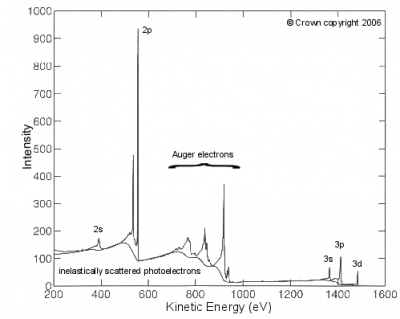
\includegraphics[width=0.6\linewidth]{img/copper.jpeg} }     

 \caption{\small \textbf{(a),(b) }Spectrum of a 10 DM coin with samarium contamination. Sm(?) refer to the shake-up and shake-off peaks also found in the pure Sm sample. \textbf{(c)} Copper spectrum. }
        \label{fig:DM}
\end{figure}

\FloatBarrier
\clearpage
 \bibliographystyle{unsrt}
\bibliography{bib}

\end{document}


